\documentclass[10pt,a4paper]{book}

\usepackage[utf8]{inputenc}
\usepackage{graphicx}

\usepackage[english]{babel}
\usepackage{amsmath}
\usepackage{amsfonts}
\usepackage{amssymb}
\author{Mohamed Abbadi}
\begin{document}
\tableofcontents


\chapter{Introduction}
\section{Games and video games}
\begin{itemize}

\item Games and video games. What is a game (definition)?\\
\item Games are grouped by genre. How many genres?\\
\item Commercial games. Mainly used for entertainment. Commercial games are \textit{big}. Commercial games society impact.\\
\item Games are not only used for entertainment.\\
\item Games are \textit{useful} for applications so-called \textit{serious}.\\
\item What is a serious game?\\
\item Examples of serious games.\\
\item What are their impact in our society?\\
\item Who build serious games (developers)?\\
\item \begin{itemize}
\item Serious developers -> description
\item Researchers -> description
\item Indie developers (special case) -> description
\end{itemize}
\item Despite their cultural impact and usefulness the above developers do not enjoy the same budget as for commercial games developers.\\
\item These budget limitations decrease the freedom for serious games developers to choose new features to implement, to investigate new interaction paradigms, to try new kind of game experience, etc.\\
\item What are these limitations?\\
\item Among the possible limitations (obstacles) we identified \textit{tools} as a big limitation.\\
\item Tools for making games are limited and not suitable.\\
\item Games are inherently complex. If we also stack to this not suitable tools then the results is dramatic in terms of complexity and expenses. Indeed many serious games projects never see the light of day.\\
\item Hence, we introduce Casanova.\\
\item Casanova is a language for making games. Casanova is aimed to reduce the complexity of the tools layer, so eventually to give serious games developers the opportunity to make games with less effort hence to increase serious games likelihood of success.

\end{itemize}


\section{Building games}
\begin{itemize}
\item discusses difficulties in building games, difficulties between AAA and research/indie games
\item tools in use
\item languages for game development
\begin{itemize}
\item Why a language? Why not a general purpose language? Inspiration from paper DS L's as  the ultimate abstraction [Paul Hudak]
\end{itemize}
\end{itemize}

\section{Problem statement}
Orchestration in games with Casanova 2
REQUIREMENTS TABLE 
\begin{center}
     \begin{tabular}{ | l | p{2cm} | p{2cm} | p{2cm}  | p{5cm} |}
     \hline
     Code & Language requirement & Run-time requirement & Name & Description \\ \hline
     R1 & Yes & No & Syntax and semantics & the language should use specific constructs designed around typical aspects present in games\\ \hline
     R2 & No & Yes & Performance & the resulted game should be fast enough to guarantee a smooth run-time experience\\ \hline
     R3 & Yes & No & Learning curve & the language should be easy to handle for novice developers \\ \hline
     R4 & Yes & No & Usability & the language should speed up development processes of those developers who master Casanova in the long-term\\ \hline
     R5 & No & Yes & Applications & the game should be run-able on the most used devices and software platforms\\ \hline
     R6 & Yes & No & Reliability & the language back-end should help developers to reduce the amount of mistakes while building games\\ \hline
     \end{tabular}
\end{center}

\subsection{Research question and process}


\subsection{Positive consequences}
...

\section{Outline}
...


\chapter{Related work}

\section{What is a game?}
\label{section_introduction}
\begin{itemize}
\item Low level, a program that indefinitely interacts with hardware components
\item High level (computer science), the derivative of the game state with respect of the time applied to the game state itself
\end{itemize}

\begin{figure}[h!]
\centering
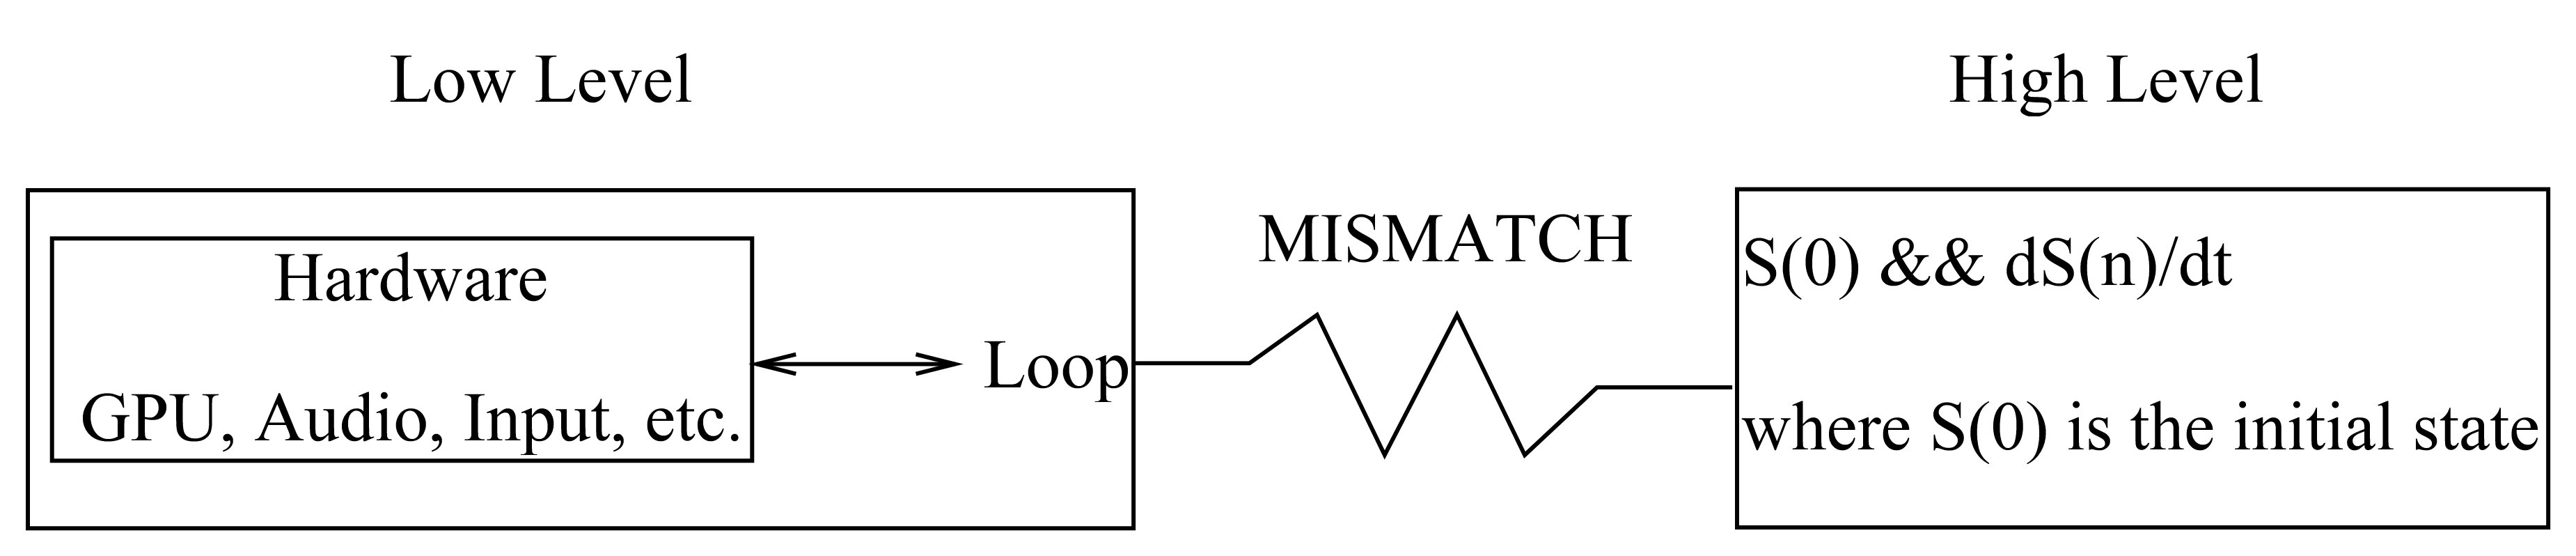
\includegraphics[scale=0.5]{Figures/games_description.png}
\caption{Game formalization (overview)}\label{game_description}
\end{figure}

\section{Game development}
\begin{itemize}
\item Research in game development tries to solve the gap/mismatch between the low level constraints and the high level description of a game.
\item \textbf{How?} Historically a hierarchy has come to life, which is described by the picture below:
\end{itemize}

\begin{figure}[h!]
\centering
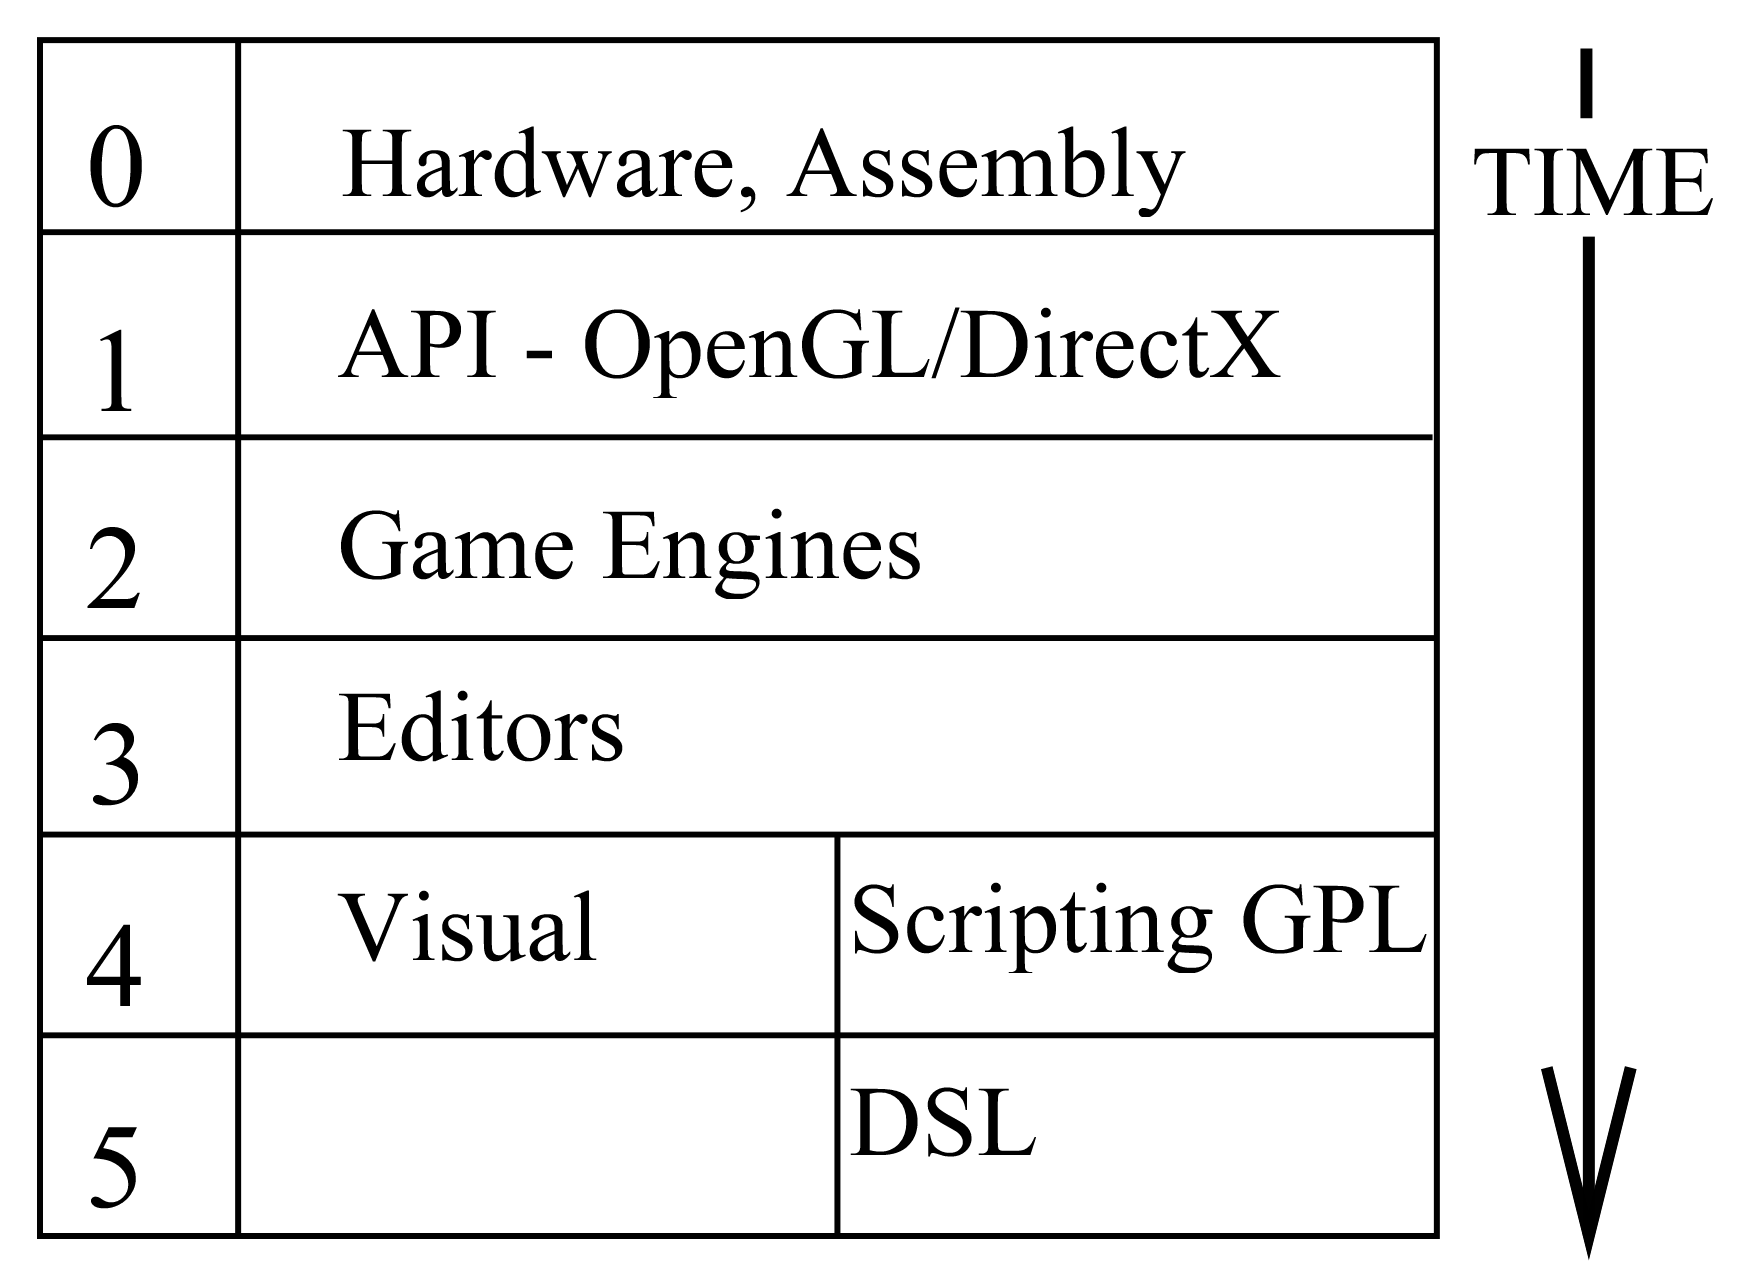
\includegraphics[scale=0.5]{Figures/game_development_evolution.png}
\caption{Game development tools evolution}\label{game_dvelopment}
\end{figure}

\newpage
\subsection{Hardware} introduction, examples (assembly games), pros, and issues
\subsection{Multimedia API} introduction, examples (DirectX, OpenGL), pros, and issues
\subsection{Engines} introduction, examples (Ogre, XNA, UnityEngine), pros, and issues
\subsection{Editors} introduction, examples (UnityEditor, UnrealEngine), pros, and issues
\subsection{Visual + GPL} introduction, examples(GameMaker,RPGmaker), pros, and issues
\subsection{DSL} introduction, examples(Casanova), pros, and issues

\section{Research questions?}
For example: 
\begin{itemize}
\item To what extent a game should be designed around the domain of games and what are the requirements
\item To what extent game development would benefit from the integration of DSLs into the development processes and to what level of abstraction
\item ...
\end{itemize}

\chapter{Requirements for general game development languages}
...

\chapter{Our proposal: the Casanova language}
FEATURES TABLE

\begin{center}
     \begin{tabular}{ | l | l | p{5cm} |}
     \hline
     Requirement & Casanova Feature & Description \\ \hline
     R1 & Casanova syntax and semantics & ... \\ \hline
     R2 & Events optimization & ... \\ \hline
     R3 & Students test & ... \\ \hline
     R4 & Usability test & ... \\ \hline
     R5 & Making games with Casanova & ... \\ \hline
     R6 & Layered compiler & ... \\ \hline
     \end{tabular}
\end{center}


\section{System description}
...
\section{Syntactic choices description}
Orchestration in games with Casanova 2 [paper]

\chapter{Language implementation and evaluation}
\section{Compiler structure}
\section{Performance optimization}
...
\subsection{State machine optimization}
Orchestration in games with Casanova 2 [paper]
\subsection{Event optimization}
High performance encapsulation in Casanova [paper]
\subsection{Event optimization and queries}
High performance encapsulation in Casanova [paper]

\chapter{Language usability and evaluation}
\section{Usability first impact}
Rotterdam usability study - [paper]
\section{Usability in depth}
Rotterdam usability study - [paper]


\chapter{Applications}
\begin{itemize}
\item Dyslexia
\item RTS
\item Contact
\item Lego
\end{itemize}

\section{Portability}
The compiler output C\# code. The Mono framework allow to run C\# code on several platform such as Windows, Linux, and Mac.


\chapter{Discussion}
...

\chapter{Conclusions}
...

\bibliography{bib}

\end{document}